\documentclass[tikz,border=10pt]{standalone}
\usepackage{tikz}
\usepackage{amsmath}

\begin{document}
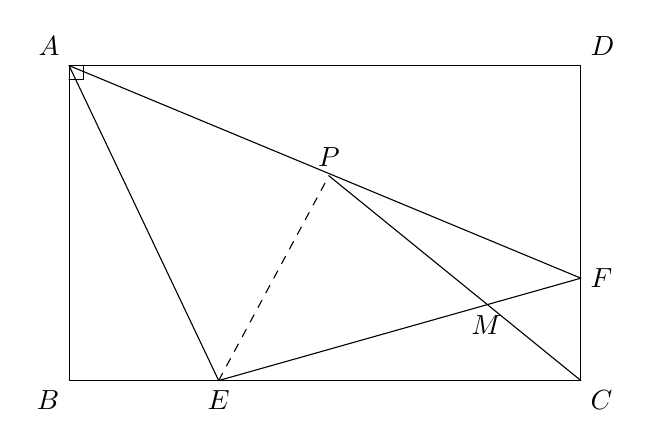
\begin{tikzpicture}[line cap=round,line join=round,scale=1]

% Coordinates
\coordinate (A) at (0,4);
\coordinate (B) at (0,0);
\coordinate (C) at (6.5,0);
\coordinate (D) at (6.5,4);
\coordinate (E) at (1.9,0);
\coordinate (F) at (6.5,1.3);
\coordinate (P) at (3.3,2.6);
\coordinate (M) at (5.3,0.95);

% Outer rectangle
\draw (A) -- (B) -- (C) -- (D) -- cycle;

% Interior segments
\draw (A) -- (E);
\draw (A) -- (F);
\draw (P) -- (C);
\draw (E) -- (F);
\draw[dashed] (E) -- (P);

% Right-angle mark at A
\draw (0.18,4) -- (0.18,3.82) -- (0,3.82);

% Labels
\node[above left] at (A) {$A$};
\node[below left] at (B) {$B$};
\node[below right] at (C) {$C$};
\node[above right] at (D) {$D$};
\node[below] at (E) {$E$};
\node[right] at (F) {$F$};
\node[above] at (P) {$P$};
\node[below] at (M) {$M$};

\end{tikzpicture}
\end{document}
